%%%%%%%%%%%%%%%%%%%%%%%%%%%%%%%%%%%%%%%%%%%%%%%%%%%%%%%%%%%%%%%%%%%%%%%%%%%%%%%%%%%%%%%%%%%%%%%%%%%%%%%%%%%%%%%%%%%%%%%%%%%%%%%%%%%%%%%%%%%%%%%%%%%%%%%%%%%%%%%%%%%
% Written By Michael Brodskiy
% Class: Fundamentals of Linear Systems
% Professor: I. Salama
%%%%%%%%%%%%%%%%%%%%%%%%%%%%%%%%%%%%%%%%%%%%%%%%%%%%%%%%%%%%%%%%%%%%%%%%%%%%%%%%%%%%%%%%%%%%%%%%%%%%%%%%%%%%%%%%%%%%%%%%%%%%%%%%%%%%%%%%%%%%%%%%%%%%%%%%%%%%%%%%%%%

\include{Includes.tex}

\title{Homework 6}
\date{\today}
\author{Michael Brodskiy\\ \small Professor: I. Salama}

\begin{document}

\maketitle

\begin{enumerate}

  \item

    \begin{enumerate}

      \item Per the rules of Laplace Transforms, we can convolve two signals by the rule that:

        $$y(t)=x_1(t)*x_2(t)\to Y(s)=X_1(s)X_2(s)$$

        As such, we may obtain:

        $$X_1(s)=\frac{1}{s+4}\quad\text{ and }\quad X_2(s)=\frac{1}{s+2}$$

        Now, we account for the shifts. We know that, for $x(t)\to x(t-t_o)$ the transform becomes $X(s)\to e^{st_o}X(s)$. Furthermore, we know that for $x(-t)\to X(-s)$. Thus, we find:

        $$X_1(s)=\frac{e^{-3s}}{-s+4}\quad\text{ and }\quad X_2(s)=\frac{e^{-2s}}{s+2}$$

        Multiplying together, we find:

        $$\boxed{Y(s)=\frac{e^{-5s}}{(4-s)(s+2)},\quad\text{ROC: } -2<\sigma<4}$$

      \item We may write this integral as the convolution of two functions:

        $$x_1(t)=\cos(2t)e^{-2t}$$
        $$x_2(t)=u(-3t+1)$$

        We now work to use the multiplicative property of the Laplace transform:

        $$\mathcal{L}\left\{ x_1(t) \right\}=\frac{s+2}{(s+2)^2+4}$$
        $$\mathcal{L}\left\{ x_2(t) \right\}=\frac{e^{-\frac{1}{3}s}}{s}$$

        We multiply the two together to get:

        $$\boxed{Y(s)=\frac{(s+2)e^{-\frac{1}{3}s}}{(s)[(s+2)^2+4]}}$$

        Note that we may also use the last property of Laplace transforms on our equation sheet to write:

        $$\int_t^{\infty} x(\tau)\,d\tau= \frac{1}{s}X(s)$$

        This gives us the same result:

        $$\boxed{Y(s)=\frac{(s+2)e^{-\frac{1}{3}s}}{(s)[(s+2)^2+4]}}$$

    \end{enumerate}

  \item

    First, we know that the poles must be at plus or minus the imaginary value, so the two poles must be at $s=-1\pm 3j$. Thus, we see that $X(s)$ can be expressed as:

    $$X(s)=\frac{k}{(s+1-3j)(s+1+3j)}$$
    $$X(s)=\frac{k}{(s+1)^2+3^2}$$

    We then apply the condition given in statement (5) to get:

    $$2=\frac{k}{(1^2)+(3^2)}$$
    $$k=20$$

    Then, because of statement (4), we know that $s=4$ is NOT in the ROC of $X(s)$. This means that we obtain the transform as:

    $$\boxed{X(s)=\frac{20}{(s+1)^2+3^2},\quad\text{ROC: }\sigma <-1}$$

    Taking the inverse transform, per our Laplace tables, we see:

    $$\boxed{x(t)=-\frac{20}{3}e^{-t}\sin(3t)u(-t)}$$

  \item

    \begin{enumerate}

      \item 

        Using our tables, we may obtain (with $X(s)$ ROC: $\sigma <3$ and $H(s)$ ROC: $\sigma>-2$):

        $$\boxed{X(s)=-\frac{5}{s-3}\quad\text{ and }H(s)=\frac{1}{s+2}}$$

      \item 

        We may write the convolution transform as:

        $$Y(s)=X(s)H(s)$$

        Thus, we get:

        $$Y(s)=\left( -\frac{5}{s-3} \right)\left( \frac{1}{s+2} \right)$$
        $$\boxed{Y(s)=-\frac{5}{(s-3)(s+2)}}$$

      \item 

        We begin by using partial fraction decomposition, which gives us:

        $$Y(s)=\frac{A}{s-3}+\frac{B}{s+2}$$

        From here, we get $A=-1$ and $B=1$, which gives us:

        $$Y(s)=\frac{-1}{s-3}+\frac{1}{s+2}$$

        Using our inverse transforms, we obtain:

        $$\boxed{y(t)=e^{3t}u(-t)+e^{-2t}u(t)}$$

      \item 

        Explicit convolution gives us:

        $$x(t)*h(t)=\int_0^t 5e^{3\tau}u(-\tau)e^{-2(t-\tau)}u(t-\tau)\,d\tau$$
        $$x(t)*h(t)=\int_0^t 5e^{-2t+5\tau}u(-\tau)u(t-\tau)\,d\tau$$

        We see that the function is bounded by:

        $$\tau \leq 0\quad\text{ and }\quad \tau\leq t$$

        From this, we may write:

        $$y(t)=-5e^t\int_0^t e^{5\tau}\,d\tau$$
        $$y(t)=-e^{-2t}\left[ e^{5\tau} \right]\Big|_0^t$$
        $$y(t)=-e^{-2t}\left[ e^{5t}-1 \right]$$

        This confirms:

        $$\boxed{y(t)=e^{3t}u(-t)+e^{-2t}u(t)}$$

    \end{enumerate}

  \item

    \begin{enumerate}

      \item 

        Taking the Laplace transform, we get:

        $$s^2Y(s)-sY(s)-6Y(s)=sX(s)$$
        $$Y(s)[s^2-s-6]=sX(s)$$
        $$\boxed{H(s)=\frac{Y(s)}{X(s)}=\frac{s}{s^2-s-6}}$$

        Thus, we see that there is a zero at $s=0$ and poles at $s=-2,3$. This allows us to plot:

        \begin{figure}[H]
          \centering
          \tikzset{every picture/.style={line width=0.75pt}} %set default line width to 0.75pt        

\begin{tikzpicture}[x=0.75pt,y=0.75pt,yscale=-1,xscale=1]
%uncomment if require: \path (0,413); %set diagram left start at 0, and has height of 413

%Shape: Axis 2D [id:dp07291137441905748] 
\draw  (271,207.4) -- (507,207.4)(294.6,4) -- (294.6,230) (500,202.4) -- (507,207.4) -- (500,212.4) (289.6,11) -- (294.6,4) -- (299.6,11)  ;
%Shape: Axis 2D [id:dp6518246903591405] 
\draw  (318.2,207.4) -- (82.2,207.4)(294.6,410.8) -- (294.6,184.8) (89.2,212.4) -- (82.2,207.4) -- (89.2,202.4) (299.6,403.8) -- (294.6,410.8) -- (289.6,403.8)  ;
%Shape: Grid [id:dp49490922295513473] 
\draw  [draw opacity=0] (294.6,57.4) -- (444.6,57.4) -- (444.6,207.4) -- (294.6,207.4) -- cycle ; \draw   (344.6,57.4) -- (344.6,207.4)(394.6,57.4) -- (394.6,207.4) ; \draw   (294.6,107.4) -- (444.6,107.4)(294.6,157.4) -- (444.6,157.4) ; \draw   (294.6,57.4) -- (444.6,57.4) -- (444.6,207.4) -- (294.6,207.4) -- cycle ;
%Shape: Grid [id:dp22016715431592204] 
\draw  [draw opacity=0] (294.6,207.4) -- (444.6,207.4) -- (444.6,357.4) -- (294.6,357.4) -- cycle ; \draw   (344.6,207.4) -- (344.6,357.4)(394.6,207.4) -- (394.6,357.4) ; \draw   (294.6,257.4) -- (444.6,257.4)(294.6,307.4) -- (444.6,307.4) ; \draw   (294.6,207.4) -- (444.6,207.4) -- (444.6,357.4) -- (294.6,357.4) -- cycle ;
%Shape: Grid [id:dp9168332724400642] 
\draw  [draw opacity=0] (144.6,207.4) -- (294.6,207.4) -- (294.6,357.4) -- (144.6,357.4) -- cycle ; \draw   (194.6,207.4) -- (194.6,357.4)(244.6,207.4) -- (244.6,357.4) ; \draw   (144.6,257.4) -- (294.6,257.4)(144.6,307.4) -- (294.6,307.4) ; \draw   (144.6,207.4) -- (294.6,207.4) -- (294.6,357.4) -- (144.6,357.4) -- cycle ;
%Shape: Grid [id:dp019661334699653366] 
\draw  [draw opacity=0] (144.6,57.4) -- (294.6,57.4) -- (294.6,207.4) -- (144.6,207.4) -- cycle ; \draw   (194.6,57.4) -- (194.6,207.4)(244.6,57.4) -- (244.6,207.4) ; \draw   (144.6,107.4) -- (294.6,107.4)(144.6,157.4) -- (294.6,157.4) ; \draw   (144.6,57.4) -- (294.6,57.4) -- (294.6,207.4) -- (144.6,207.4) -- cycle ;
%Shape: Circle [id:dp8466727816697135] 
\draw  [line width=1.5]  (289.15,207.4) .. controls (289.15,204.39) and (291.59,201.95) .. (294.6,201.95) .. controls (297.61,201.95) and (300.05,204.39) .. (300.05,207.4) .. controls (300.05,210.41) and (297.61,212.85) .. (294.6,212.85) .. controls (291.59,212.85) and (289.15,210.41) .. (289.15,207.4) -- cycle ;
%Straight Lines [id:da019164220491805106] 
\draw [line width=1.5]    (202.22,200.28) -- (187.78,214.72) ;
%Straight Lines [id:da7010872252517704] 
\draw [line width=1.5]    (202.22,214.72) -- (187.78,200.28) ;

%Straight Lines [id:da8787997404879367] 
\draw [line width=1.5]    (452.22,200.28) -- (437.78,214.72) ;
%Straight Lines [id:da40962171693247995] 
\draw [line width=1.5]    (452.22,214.72) -- (437.78,200.28) ;

%Curve Lines [id:da12390900966481411] 
\draw  [dash pattern={on 4.5pt off 4.5pt}]  (117,246) .. controls (156.6,216.3) and (147.2,249.33) .. (185.81,220.88) ;
\draw [shift={(187,220)}, rotate = 143.13] [color={rgb, 255:red, 0; green, 0; blue, 0 }  ][line width=0.75]    (10.93,-3.29) .. controls (6.95,-1.4) and (3.31,-0.3) .. (0,0) .. controls (3.31,0.3) and (6.95,1.4) .. (10.93,3.29)   ;
%Curve Lines [id:da10550563739707763] 
\draw  [dash pattern={on 4.5pt off 4.5pt}]  (528.22,170.28) .. controls (488.62,199.98) and (498.03,166.95) .. (459.41,195.4) ;
\draw [shift={(458.22,196.28)}, rotate = 323.13] [color={rgb, 255:red, 0; green, 0; blue, 0 }  ][line width=0.75]    (10.93,-3.29) .. controls (6.95,-1.4) and (3.31,-0.3) .. (0,0) .. controls (3.31,0.3) and (6.95,1.4) .. (10.93,3.29)   ;

% Text Node
\draw (302,3.4) node [anchor=north west][inner sep=0.75pt]    {$\omega $};
% Text Node
\draw (507,209.4) node [anchor=north west][inner sep=0.75pt]    {$\sigma $};
% Text Node
\draw (26,249) node [anchor=north west][inner sep=0.75pt]   [align=left] {Pole: $\displaystyle \sigma =-2$};
% Text Node
\draw (528.22,167.28) node [anchor=south] [inner sep=0.75pt]   [align=left] {Pole: $\displaystyle \sigma =3$};
% Text Node
\draw (246.6,160.4) node [anchor=north west][inner sep=0.75pt]   [align=left] {Hole:\\$\displaystyle s=0$};


\end{tikzpicture}

          \caption{Pole-Zero Plot}
          \label{fig:1}
        \end{figure}
        
      \item 

        We may begin by using partial fraction decomposition:

        $$\frac{s}{s^2-s-6}\Rightarrow \frac{A}{s-3}+\frac{B}{s+2}$$

        Plugging in our values, we find $A=3/5$ and $B=2/5$, which gives us:

        $$H(s)=\frac{3/5}{s-3}+\frac{2/5}{s+2}$$

        \begin{enumerate}

          \item When the system is stable, we know that the ROC must be bounded. Thus, we know that the ROC is $-2<\sigma<3$. Using our transform table, this gives:

            $$\boxed{h(t)=-\frac{3}{5}e^{3t}u(-t)+\frac{2}{5}e^{-2t}u(t)}$$

          \item When the system is causal, we know that the ROC is right-sided, such that $\sigma>3$. Thus, we see:

            $$\boxed{h(t)=\frac{3}{5}e^{3t}u(t)+\frac{2}{5}e^{-2t}u(t)}$$

          \item When it is neither stable nor causal, the ROC must be left-sided and can not include the j$\omega$ axis. This gives us:

            $$\boxed{h(t)=\frac{3}{5}e^{3t}u(t)-\frac{2}{5}e^{-2t}u(-t)}$$

        \end{enumerate}

    \end{enumerate}

  \item Given that this is the step response, and that it is multiplied by the step function, we know that:

    $$X(s)=\frac{1}{s}$$

    We take the transform of $y(t)$ to get:

    $$Y(s)=\frac{1}{s}-\frac{1}{s+2}-\frac{2}{(s+2)^2}$$

    We know that:

    $$H(s)=\frac{Y(s)}{H(s)}$$

    Thus, we find the transfer function be:

    $$H(s)=1-\frac{s}{s+2}-\frac{2s}{(s+2)^2}$$
    $$H(s)=\frac{4}{(s+2)^2}$$

    Then we can find:

    $$Y_1(s)=\frac{1}{s}-\frac{2}{s+2}+\frac{1}{s+4}$$

    Knowing that this must be equivalent to the transfer function, we see:

    $$\frac{Y_1(s)}{H(s)}=X_1(s)$$

    This gives us:

    $$X_1(s)=\frac{(s+2)^2}{4s}-.5(s+2)+\frac{(s+2)^2}{4(s+4)}$$
    $$X_1(s)=\frac{(s+2)^2}{4s}-.5(s+2)+\frac{(s+2)^2}{4s+16}$$

    We can simplify to get:

    $$X_1(s)=\frac{2s+4}{s^2+4s}$$
    $$X_1(s)=\frac{2}{s+4}+\frac{4}{s(s+4)}$$

    We use partial fraction decomposition for the second term to get:

    $$X_1(s)=\frac{2}{s+4}+\frac{A}{s+4}+\frac{B}{s}$$

    We find $A=-1$ and $B=1$ to get:

    $$X_1(s)=\frac{1}{s+4}+\frac{1}{s}$$

    Taking the inverse, we find:

    $$\boxed{x_1(t)=[e^{-4t}+1]u(t)}$$

  \item

    We may express $x(t)$ as:

    $$x(t)=e^{t}u(-t)+e^{-t}u(t)$$

    This gives us:

    $$X(s)=-\frac{1}{s-1}+\frac{1}{s+1}$$

    We combine the two terms to get:

    $$X(s)=\frac{-2}{s^2-1}$$

    Multiplying by the system function, we get:

    $$Y(s)=\left[ \frac{s+1}{s^2+2s+9} \right]\left[ -\frac{2}{s^2-1} \right]$$

    We continue to simplify:

    $$Y(s)=\left[ \frac{1}{s^2+2s+9} \right]\left[ -\frac{2}{s-1} \right]$$
    $$Y(s)=\frac{-2}{(s^2+2s+9)(s-1)}$$

    We then use partial fraction decomposition to write:

    $$Y(s)=\frac{A}{s-1}+\frac{Bs+C}{s^2+2s+9}$$

    Thus, we get:

    $$A(s^2+2s+9)+(Bs+C)(s-1)=-2$$
    $$As^2+2As+9A+Bs^2-Bs+Cs-C=-2$$

    From this, we can set up the following system:

    $$A+B=0$$
    $$2A-B-C=0$$
    $$9A-C=-2$$

    Solving the system, we see: $A=-\frac{1}{6}$, $B=\frac{1}{6}$, and $C=\frac{1}{2}$, which gives us:

    $$Y(s)=\frac{-1/6}{s-1}+\frac{(1/6)s+(1/2)}{s^2+2s+9}$$

    We break this up further to see:

    $$Y(s)=\frac{-1/6}{s-1}+\frac{(1/6)s+(1/6)}{(s+1)^2+8}+\frac{(1/3)}{(s+1)^2+8}$$
    $$Y(s)=\frac{-1/6}{s-1}+\frac{(1/6)s+(1/6)}{(s+1)^2+8}+\frac{1}{\sqrt{8}}\frac{3\sqrt{8}}{(s+1)^2+8}$$

    We then use the Laplace tables, and the fact that the system is causal, to get:

    $$\boxed{y(t)=-\frac{1}{6}e^{t}u(t)+\frac{1}{6}e^{-t}\cos(\sqrt{8}t)u(t)+\frac{1}{3\sqrt{8}}e^{-t}\sin(\sqrt{8}t)u(t)}$$

  \item

    \begin{enumerate}

      \item We may observe that the left side of the diagram indicates poles, and the right side indicates zeros, while the $s^{-1}$ blocks are delays. We know that the transfer function may be written as:

        $$H(s)=\dfrac{\displaystyle \sum_{n=0}^Nb_ns^{-n}}{\displaystyle 1+\sum_{n=1}^{N}a_ns^{-n}}$$

        We may see that $N=2$, which gives us:

        $$H(s)=\dfrac{\displaystyle \sum_{n=0}^2b_ns^{-n}}{\displaystyle 1+\sum_{n=1}^{2}-a_ns^{-n}}$$

        First, we work to get the numerator:

        $$H(s)=\frac{1-s^{-1}-3s^{-2}}{1+\sum_{n=1}^{2}a_ns^{-n}}$$

        And then the denominator:

        $$H(s)=\frac{1-s^{-1}-3s^{-2}}{1+2s^{-1}+4s^{-2}}$$

        Multiplying both the numerator and denominator by $s^2$, we get:

        $$H(s)=\frac{s^2-s-3}{s^2+2s+4}$$

        We know that the transfer function is equivalent to:

        $$H(s)=\frac{Y(s)}{X(s)}$$

        This allows us to obtain the following:

        $$s^2X(s)-sX(s)-3X(s)=s^2Y(s)+2sY(s)+4Y(s)$$

        Taking the invers transform, we see:

        $$\boxed{\frac{d^2y(t)}{dt^2}+2\frac{dy(t)}{dt}+4y(t)=\frac{d^2x(t)}{dt^2}-\frac{dx(t)}{dt}-3x(t)}$$

      \item We know the system is stable if all poles are to the left of the $s$-plane. This gives us:

        $$s^2+2s+4=0$$

        Using the quadratic equation, we get:

        $$s=\frac{-2\pm\sqrt{4-4(1)(4)}}{2}$$
        $$s=-1\pm 3j$$

        Given the $-1$ real part, all poles are to the left of the $s$-plane, and, therefore, the \underline{system is stable}.

    \end{enumerate}

  \item

    \begin{enumerate}

      \item From the information,  we know $Y(s)=(2s^2+3s-4)Y_1(s)$, which allows us to write:

        $$\boxed{y(t)=2\frac{d^2y_1(t)}{dt^2}+3\frac{dy_1(t)}{dt}-4y_1(t)}$$

      \item From the figure, we may observe the following relationship:

        $$s^{-1}f(t)=y_1(t)$$

        This allows us to obtain:

        $$\boxed{f(t)=\frac{dy_1(t)}{dt}}$$

      \item Similar to part (b), we may observe the flow of the diagram to see:

        $$s^{-2}e(t)=y_1(t)$$
        $$e(t)=s^2y_1(t)$$

        This allows us to get:

        $$\boxed{e(t)=\frac{d^2y_1(t)}{dt^2}}$$

      \item Given parts (a), (b), and (c), we may write the original signal as:

        $$\boxed{y(t)=2e(t)+3f(t)-4y_1(t)}$$

      \item 

        We may combine the diagram and result from (d) to form the following figure:

        \begin{figure}[H]
          \centering
          \tikzset{every picture/.style={line width=0.75pt}} %set default line width to 0.75pt        

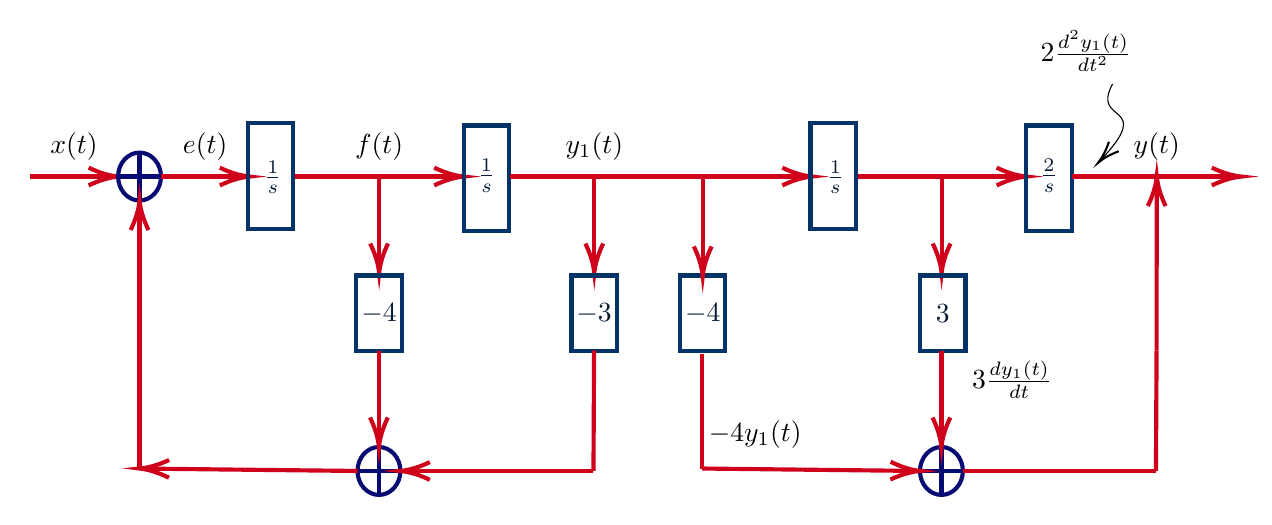
\begin{tikzpicture}[x=0.75pt,y=0.75pt,yscale=-1,xscale=1]
%uncomment if require: \path (0,413); %set diagram left start at 0, and has height of 413

%Straight Lines [id:da802785846498601] 
\draw [color={rgb, 255:red, 208; green, 2; blue, 27 }  ,draw opacity=1 ][line width=1.5]    (35.29,110.61) -- (74.86,110.61) ;
\draw [shift={(77.86,110.61)}, rotate = 180] [color={rgb, 255:red, 208; green, 2; blue, 27 }  ,draw opacity=1 ][line width=1.5]    (14.21,-4.28) .. controls (9.04,-1.82) and (4.3,-0.39) .. (0,0) .. controls (4.3,0.39) and (9.04,1.82) .. (14.21,4.28)   ;
%Flowchart: Or [id:dp553678149380639] 
\draw  [color={rgb, 255:red, 7; green, 11; blue, 114 }  ,draw opacity=1 ][line width=1.5]  (77.86,110.61) .. controls (77.86,104.24) and (82.48,99.07) .. (88.19,99.07) .. controls (93.89,99.07) and (98.51,104.24) .. (98.51,110.61) .. controls (98.51,116.99) and (93.89,122.16) .. (88.19,122.16) .. controls (82.48,122.16) and (77.86,116.99) .. (77.86,110.61) -- cycle ; \draw  [color={rgb, 255:red, 7; green, 11; blue, 114 }  ,draw opacity=1 ][line width=1.5]  (77.86,110.61) -- (98.51,110.61) ; \draw  [color={rgb, 255:red, 7; green, 11; blue, 114 }  ,draw opacity=1 ][line width=1.5]  (88.19,99.07) -- (88.19,122.16) ;
%Straight Lines [id:da0005729357145491942] 
\draw [color={rgb, 255:red, 208; green, 2; blue, 27 }  ,draw opacity=1 ][line width=1.5]    (98.51,110.61) -- (138.08,110.61) ;
\draw [shift={(141.08,110.61)}, rotate = 180] [color={rgb, 255:red, 208; green, 2; blue, 27 }  ,draw opacity=1 ][line width=1.5]    (14.21,-4.28) .. controls (9.04,-1.82) and (4.3,-0.39) .. (0,0) .. controls (4.3,0.39) and (9.04,1.82) .. (14.21,4.28)   ;
%Straight Lines [id:da3637837568605653] 
\draw [color={rgb, 255:red, 208; green, 2; blue, 27 }  ,draw opacity=1 ][line width=1.5]    (162.9,110.61) -- (241.34,110.61) ;
\draw [shift={(244.34,110.61)}, rotate = 180] [color={rgb, 255:red, 208; green, 2; blue, 27 }  ,draw opacity=1 ][line width=1.5]    (14.21,-4.28) .. controls (9.04,-1.82) and (4.3,-0.39) .. (0,0) .. controls (4.3,0.39) and (9.04,1.82) .. (14.21,4.28)   ;
%Straight Lines [id:da7853547776401528] 
\draw [color={rgb, 255:red, 208; green, 2; blue, 27 }  ,draw opacity=1 ][line width=1.5]    (203.62,110.61) -- (203.62,154.09) ;
\draw [shift={(203.62,157.09)}, rotate = 270] [color={rgb, 255:red, 208; green, 2; blue, 27 }  ,draw opacity=1 ][line width=1.5]    (14.21,-4.28) .. controls (9.04,-1.82) and (4.3,-0.39) .. (0,0) .. controls (4.3,0.39) and (9.04,1.82) .. (14.21,4.28)   ;
%Shape: Rectangle [id:dp7429901223650903] 
\draw  [color={rgb, 255:red, 4; green, 51; blue, 104 }  ,draw opacity=1 ][line width=1.5]  (244.45,86) -- (266.27,86) -- (266.27,137) -- (244.45,137) -- cycle ;
%Straight Lines [id:da5727032991915001] 
\draw [color={rgb, 255:red, 208; green, 2; blue, 27 }  ,draw opacity=1 ][line width=1.5]    (266.56,110.61) -- (369.51,110.61) ;
%Straight Lines [id:da9679330996422791] 
\draw [color={rgb, 255:red, 208; green, 2; blue, 27 }  ,draw opacity=1 ][line width=1.5]    (307.28,110.61) -- (307.28,154.09) ;
\draw [shift={(307.28,157.09)}, rotate = 270] [color={rgb, 255:red, 208; green, 2; blue, 27 }  ,draw opacity=1 ][line width=1.5]    (14.21,-4.28) .. controls (9.04,-1.82) and (4.3,-0.39) .. (0,0) .. controls (4.3,0.39) and (9.04,1.82) .. (14.21,4.28)   ;
%Shape: Rectangle [id:dp8462678044175708] 
\draw  [color={rgb, 255:red, 4; green, 51; blue, 104 }  ,draw opacity=1 ][line width=1.5]  (192.62,158.27) -- (214.44,158.27) -- (214.44,194.75) -- (192.62,194.75) -- cycle ;
%Shape: Rectangle [id:dp21684179070571108] 
\draw  [color={rgb, 255:red, 4; green, 51; blue, 104 }  ,draw opacity=1 ][line width=1.5]  (296.28,158.27) -- (318.1,158.27) -- (318.1,194.75) -- (296.28,194.75) -- cycle ;
%Flowchart: Or [id:dp24510455676250775] 
\draw  [color={rgb, 255:red, 7; green, 11; blue, 114 }  ,draw opacity=1 ][line width=1.5]  (193.21,252.46) .. controls (193.21,246.08) and (197.83,240.92) .. (203.53,240.92) .. controls (209.24,240.92) and (213.86,246.08) .. (213.86,252.46) .. controls (213.86,258.83) and (209.24,264) .. (203.53,264) .. controls (197.83,264) and (193.21,258.83) .. (193.21,252.46) -- cycle ; \draw  [color={rgb, 255:red, 7; green, 11; blue, 114 }  ,draw opacity=1 ][line width=1.5]  (193.21,252.46) -- (213.86,252.46) ; \draw  [color={rgb, 255:red, 7; green, 11; blue, 114 }  ,draw opacity=1 ][line width=1.5]  (203.53,240.92) -- (203.53,264) ;
%Straight Lines [id:da743736925871232] 
\draw [color={rgb, 255:red, 208; green, 2; blue, 27 }  ,draw opacity=1 ][line width=1.5]    (203.53,194.44) -- (203.53,237.92) ;
\draw [shift={(203.53,240.92)}, rotate = 270] [color={rgb, 255:red, 208; green, 2; blue, 27 }  ,draw opacity=1 ][line width=1.5]    (14.21,-4.28) .. controls (9.04,-1.82) and (4.3,-0.39) .. (0,0) .. controls (4.3,0.39) and (9.04,1.82) .. (14.21,4.28)   ;
%Straight Lines [id:da4445130041220482] 
\draw [color={rgb, 255:red, 208; green, 2; blue, 27 }  ,draw opacity=1 ][line width=1.5]    (307.19,194.38) -- (306.89,252.46) ;
%Straight Lines [id:da16757916335619527] 
\draw [color={rgb, 255:red, 208; green, 2; blue, 27 }  ,draw opacity=1 ][line width=1.5]    (306.89,252.46) -- (216.86,252.46) ;
\draw [shift={(213.86,252.46)}, rotate = 360] [color={rgb, 255:red, 208; green, 2; blue, 27 }  ,draw opacity=1 ][line width=1.5]    (14.21,-4.28) .. controls (9.04,-1.82) and (4.3,-0.39) .. (0,0) .. controls (4.3,0.39) and (9.04,1.82) .. (14.21,4.28)   ;
%Straight Lines [id:da06342954948494517] 
\draw [color={rgb, 255:red, 208; green, 2; blue, 27 }  ,draw opacity=1 ][line width=1.5]    (193.21,252.46) -- (91.19,251.32) ;
\draw [shift={(88.19,251.28)}, rotate = 0.64] [color={rgb, 255:red, 208; green, 2; blue, 27 }  ,draw opacity=1 ][line width=1.5]    (14.21,-4.28) .. controls (9.04,-1.82) and (4.3,-0.39) .. (0,0) .. controls (4.3,0.39) and (9.04,1.82) .. (14.21,4.28)   ;
%Straight Lines [id:da9868110229846314] 
\draw [color={rgb, 255:red, 208; green, 2; blue, 27 }  ,draw opacity=1 ][line width=1.5]    (88.19,251.28) -- (88.19,125.16) ;
\draw [shift={(88.19,122.16)}, rotate = 90] [color={rgb, 255:red, 208; green, 2; blue, 27 }  ,draw opacity=1 ][line width=1.5]    (14.21,-4.28) .. controls (9.04,-1.82) and (4.3,-0.39) .. (0,0) .. controls (4.3,0.39) and (9.04,1.82) .. (14.21,4.28)   ;
%Shape: Rectangle [id:dp5674177228326189] 
\draw  [color={rgb, 255:red, 4; green, 51; blue, 104 }  ,draw opacity=1 ][line width=1.5]  (140.45,85) -- (162.27,85) -- (162.27,136) -- (140.45,136) -- cycle ;
%Straight Lines [id:da6353712181396247] 
\draw [color={rgb, 255:red, 208; green, 2; blue, 27 }  ,draw opacity=1 ][line width=1.5]    (369.51,110.61) -- (409.08,110.61) ;
\draw [shift={(412.08,110.61)}, rotate = 180] [color={rgb, 255:red, 208; green, 2; blue, 27 }  ,draw opacity=1 ][line width=1.5]    (14.21,-4.28) .. controls (9.04,-1.82) and (4.3,-0.39) .. (0,0) .. controls (4.3,0.39) and (9.04,1.82) .. (14.21,4.28)   ;
%Straight Lines [id:da5829042456704695] 
\draw [color={rgb, 255:red, 208; green, 2; blue, 27 }  ,draw opacity=1 ][line width=1.5]    (433.9,110.61) -- (512.34,110.61) ;
\draw [shift={(515.34,110.61)}, rotate = 180] [color={rgb, 255:red, 208; green, 2; blue, 27 }  ,draw opacity=1 ][line width=1.5]    (14.21,-4.28) .. controls (9.04,-1.82) and (4.3,-0.39) .. (0,0) .. controls (4.3,0.39) and (9.04,1.82) .. (14.21,4.28)   ;
%Straight Lines [id:da9215072887229189] 
\draw [color={rgb, 255:red, 208; green, 2; blue, 27 }  ,draw opacity=1 ][line width=1.5]    (474.62,110.61) -- (474.62,154.09) ;
\draw [shift={(474.62,157.09)}, rotate = 270] [color={rgb, 255:red, 208; green, 2; blue, 27 }  ,draw opacity=1 ][line width=1.5]    (14.21,-4.28) .. controls (9.04,-1.82) and (4.3,-0.39) .. (0,0) .. controls (4.3,0.39) and (9.04,1.82) .. (14.21,4.28)   ;
%Shape: Rectangle [id:dp2516520568905628] 
\draw  [color={rgb, 255:red, 4; green, 51; blue, 104 }  ,draw opacity=1 ][line width=1.5]  (515.45,86) -- (537.27,86) -- (537.27,137) -- (515.45,137) -- cycle ;
%Straight Lines [id:da4261405254199824] 
\draw [color={rgb, 255:red, 208; green, 2; blue, 27 }  ,draw opacity=1 ][line width=1.5]    (537.56,110.61) -- (616,110.61) ;
\draw [shift={(619,110.61)}, rotate = 180] [color={rgb, 255:red, 208; green, 2; blue, 27 }  ,draw opacity=1 ][line width=1.5]    (14.21,-4.28) .. controls (9.04,-1.82) and (4.3,-0.39) .. (0,0) .. controls (4.3,0.39) and (9.04,1.82) .. (14.21,4.28)   ;
%Straight Lines [id:da6251012152063772] 
\draw [color={rgb, 255:red, 208; green, 2; blue, 27 }  ,draw opacity=1 ][line width=1.5]    (578.28,113.61) -- (578.19,194.38) ;
\draw [shift={(578.28,110.61)}, rotate = 90.06] [color={rgb, 255:red, 208; green, 2; blue, 27 }  ,draw opacity=1 ][line width=1.5]    (14.21,-4.28) .. controls (9.04,-1.82) and (4.3,-0.39) .. (0,0) .. controls (4.3,0.39) and (9.04,1.82) .. (14.21,4.28)   ;
%Shape: Rectangle [id:dp1355970092994433] 
\draw  [color={rgb, 255:red, 4; green, 51; blue, 104 }  ,draw opacity=1 ][line width=1.5]  (348.62,158.27) -- (370.44,158.27) -- (370.44,194.75) -- (348.62,194.75) -- cycle ;
%Shape: Rectangle [id:dp6823121378438627] 
\draw  [color={rgb, 255:red, 4; green, 51; blue, 104 }  ,draw opacity=1 ][line width=1.5]  (464.28,158.27) -- (486.1,158.27) -- (486.1,194.75) -- (464.28,194.75) -- cycle ;
%Flowchart: Or [id:dp7661436109510428] 
\draw  [color={rgb, 255:red, 7; green, 11; blue, 114 }  ,draw opacity=1 ][line width=1.5]  (464.21,252.46) .. controls (464.21,246.08) and (468.83,240.92) .. (474.53,240.92) .. controls (480.24,240.92) and (484.86,246.08) .. (484.86,252.46) .. controls (484.86,258.83) and (480.24,264) .. (474.53,264) .. controls (468.83,264) and (464.21,258.83) .. (464.21,252.46) -- cycle ; \draw  [color={rgb, 255:red, 7; green, 11; blue, 114 }  ,draw opacity=1 ][line width=1.5]  (464.21,252.46) -- (484.86,252.46) ; \draw  [color={rgb, 255:red, 7; green, 11; blue, 114 }  ,draw opacity=1 ][line width=1.5]  (474.53,240.92) -- (474.53,264) ;
%Straight Lines [id:da01912398853988273] 
\draw [color={rgb, 255:red, 208; green, 2; blue, 27 }  ,draw opacity=1 ][line width=1.5]    (474.53,194.44) -- (474.53,237.92) ;
\draw [shift={(474.53,240.92)}, rotate = 270] [color={rgb, 255:red, 208; green, 2; blue, 27 }  ,draw opacity=1 ][line width=1.5]    (14.21,-4.28) .. controls (9.04,-1.82) and (4.3,-0.39) .. (0,0) .. controls (4.3,0.39) and (9.04,1.82) .. (14.21,4.28)   ;
%Straight Lines [id:da8678617048496559] 
\draw [color={rgb, 255:red, 208; green, 2; blue, 27 }  ,draw opacity=1 ][line width=1.5]    (578.19,194.38) -- (577.89,252.46) ;
%Straight Lines [id:da4878156257526778] 
\draw [color={rgb, 255:red, 208; green, 2; blue, 27 }  ,draw opacity=1 ][line width=1.5]    (577.89,252.46) -- (484.86,252.46) ;
%Straight Lines [id:da01710459462168179] 
\draw [color={rgb, 255:red, 208; green, 2; blue, 27 }  ,draw opacity=1 ][line width=1.5]    (461.21,252.43) -- (359.19,251.28) ;
\draw [shift={(464.21,252.46)}, rotate = 180.64] [color={rgb, 255:red, 208; green, 2; blue, 27 }  ,draw opacity=1 ][line width=1.5]    (14.21,-4.28) .. controls (9.04,-1.82) and (4.3,-0.39) .. (0,0) .. controls (4.3,0.39) and (9.04,1.82) .. (14.21,4.28)   ;
%Straight Lines [id:da46828292830077667] 
\draw [color={rgb, 255:red, 208; green, 2; blue, 27 }  ,draw opacity=1 ][line width=1.5]    (359.19,251.28) -- (359.19,196.16) ;
%Shape: Rectangle [id:dp706545784774389] 
\draw  [color={rgb, 255:red, 4; green, 51; blue, 104 }  ,draw opacity=1 ][line width=1.5]  (411.45,85) -- (433.27,85) -- (433.27,136) -- (411.45,136) -- cycle ;
%Straight Lines [id:da3449564708681504] 
\draw [color={rgb, 255:red, 208; green, 2; blue, 27 }  ,draw opacity=1 ][line width=1.5]    (359.53,155.51) -- (359.53,111.38) ;
\draw [shift={(359.53,158.51)}, rotate = 270] [color={rgb, 255:red, 208; green, 2; blue, 27 }  ,draw opacity=1 ][line width=1.5]    (14.21,-4.28) .. controls (9.04,-1.82) and (4.3,-0.39) .. (0,0) .. controls (4.3,0.39) and (9.04,1.82) .. (14.21,4.28)   ;
%Curve Lines [id:da4275503219374158] 
\draw    (557,66) .. controls (546.17,85.7) and (578.02,74.35) .. (551.26,102.68) ;
\draw [shift={(550,104)}, rotate = 314.03] [color={rgb, 255:red, 0; green, 0; blue, 0 }  ][line width=0.75]    (10.93,-3.29) .. controls (6.95,-1.4) and (3.31,-0.3) .. (0,0) .. controls (3.31,0.3) and (6.95,1.4) .. (10.93,3.29)   ;

% Text Node
\draw (56.57,104.21) node [anchor=south] [inner sep=0.75pt]    {$x( t)$};
% Text Node
\draw (119.8,104.21) node [anchor=south] [inner sep=0.75pt]    {$e( t)$};
% Text Node
\draw (152.39,110.99) node  [color={rgb, 255:red, 5; green, 27; blue, 53 }  ,opacity=1 ]  {$\frac{1}{s}$};
% Text Node
\draw (203.62,104.21) node [anchor=south] [inner sep=0.75pt]    {$f( t)$};
% Text Node
\draw (255.36,110.24) node  [color={rgb, 255:red, 5; green, 27; blue, 53 }  ,opacity=1 ]  {$\frac{1}{s}$};
% Text Node
\draw (307.28,104.21) node [anchor=south] [inner sep=0.75pt]    {$y_{1}( t)$};
% Text Node
\draw (203.53,176.51) node  [color={rgb, 255:red, 5; green, 27; blue, 53 }  ,opacity=1 ]  {$-4$};
% Text Node
\draw (307.19,176.51) node  [color={rgb, 255:red, 5; green, 27; blue, 53 }  ,opacity=1 ]  {$-3$};
% Text Node
\draw (423.39,110.99) node  [color={rgb, 255:red, 5; green, 27; blue, 53 }  ,opacity=1 ]  {$\frac{1}{s}$};
% Text Node
\draw (526.36,110.24) node  [color={rgb, 255:red, 5; green, 27; blue, 53 }  ,opacity=1 ]  {$\frac{2}{s}$};
% Text Node
\draw (578.28,104.21) node [anchor=south] [inner sep=0.75pt]    {$y( t)$};
% Text Node
\draw (359.53,176.51) node  [color={rgb, 255:red, 5; green, 27; blue, 53 }  ,opacity=1 ]  {$-4$};
% Text Node
\draw (475.19,176.51) node  [color={rgb, 255:red, 5; green, 27; blue, 53 }  ,opacity=1 ]  {$3$};
% Text Node
\draw (361.19,227.12) node [anchor=north west][inner sep=0.75pt]    {$-4y_{1}( t)$};
% Text Node
\draw (488.1,198.15) node [anchor=north west][inner sep=0.75pt]    {$3\frac{dy_{1}( t)}{dt}$};
% Text Node
\draw (521.1,39.15) node [anchor=north west][inner sep=0.75pt]    {$2\frac{d^{2} y_{1}( t)}{dt^{2}}$};


\end{tikzpicture}

          \caption{Full System $(S)$ Diagram}
          \label{fig:2}
        \end{figure}

      \item From the provided form, we may write:

        $$H_1(s)=\frac{Y_1(s)}{X(s)}\quad\text{ and }\quad H_2(s)=\frac{Y(s)}{Y_1(s)}$$

        This gives us:

        $$(s+3)Y_1(s)=(2s-4)X(s)\Rightarrow (s+2)Y_1(s)=(s+1)Y(s)$$
        $$\frac{dy_1(t)}{dt}+3y_1(t)=2\frac{dx(t)}{dt}-4x(t)\Rightarrow \frac{dy_1(t)}{dt}+2y_1(t)=\frac{dy(t)}{dt}+y(t)$$

        From $H_2(s)$, we may obtain:

        \begin{figure}[H]
          \centering
          \tikzset{every picture/.style={line width=0.75pt}} %set default line width to 0.75pt        

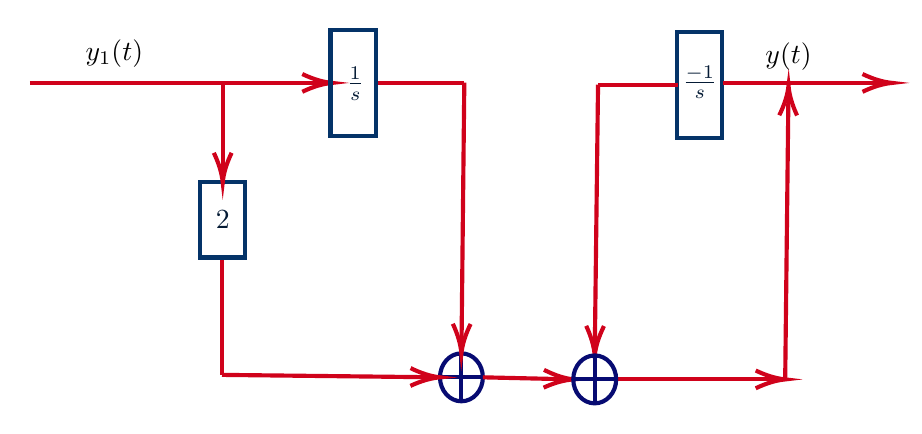
\begin{tikzpicture}[x=0.75pt,y=0.75pt,yscale=-1,xscale=1]
%uncomment if require: \path (0,413); %set diagram left start at 0, and has height of 413

%Straight Lines [id:da5727032991915001] 
\draw [color={rgb, 255:red, 208; green, 2; blue, 27 }  ,draw opacity=1 ][line width=1.5]    (58.56,110.61) -- (161.51,110.61) ;
%Straight Lines [id:da6353712181396247] 
\draw [color={rgb, 255:red, 208; green, 2; blue, 27 }  ,draw opacity=1 ][line width=1.5]    (161.51,110.61) -- (201.08,110.61) ;
\draw [shift={(204.08,110.61)}, rotate = 180] [color={rgb, 255:red, 208; green, 2; blue, 27 }  ,draw opacity=1 ][line width=1.5]    (14.21,-4.28) .. controls (9.04,-1.82) and (4.3,-0.39) .. (0,0) .. controls (4.3,0.39) and (9.04,1.82) .. (14.21,4.28)   ;
%Straight Lines [id:da5829042456704695] 
\draw [color={rgb, 255:red, 208; green, 2; blue, 27 }  ,draw opacity=1 ][line width=1.5]    (341.09,253.46) -- (419.53,253.46) ;
\draw [shift={(422.53,253.46)}, rotate = 180] [color={rgb, 255:red, 208; green, 2; blue, 27 }  ,draw opacity=1 ][line width=1.5]    (14.21,-4.28) .. controls (9.04,-1.82) and (4.3,-0.39) .. (0,0) .. controls (4.3,0.39) and (9.04,1.82) .. (14.21,4.28)   ;
%Shape: Rectangle [id:dp2516520568905628] 
\draw  [color={rgb, 255:red, 4; green, 51; blue, 104 }  ,draw opacity=1 ][line width=1.5]  (370.45,86) -- (392.27,86) -- (392.27,137) -- (370.45,137) -- cycle ;
%Straight Lines [id:da4261405254199824] 
\draw [color={rgb, 255:red, 208; green, 2; blue, 27 }  ,draw opacity=1 ][line width=1.5]    (392.56,110.61) -- (471,110.61) ;
\draw [shift={(474,110.61)}, rotate = 180] [color={rgb, 255:red, 208; green, 2; blue, 27 }  ,draw opacity=1 ][line width=1.5]    (14.21,-4.28) .. controls (9.04,-1.82) and (4.3,-0.39) .. (0,0) .. controls (4.3,0.39) and (9.04,1.82) .. (14.21,4.28)   ;
%Shape: Rectangle [id:dp1355970092994433] 
\draw  [color={rgb, 255:red, 4; green, 51; blue, 104 }  ,draw opacity=1 ][line width=1.5]  (140.62,158.27) -- (162.44,158.27) -- (162.44,194.75) -- (140.62,194.75) -- cycle ;
%Flowchart: Or [id:dp7661436109510428] 
\draw  [color={rgb, 255:red, 7; green, 11; blue, 114 }  ,draw opacity=1 ][line width=1.5]  (256.21,252.46) .. controls (256.21,246.08) and (260.83,240.92) .. (266.53,240.92) .. controls (272.24,240.92) and (276.86,246.08) .. (276.86,252.46) .. controls (276.86,258.83) and (272.24,264) .. (266.53,264) .. controls (260.83,264) and (256.21,258.83) .. (256.21,252.46) -- cycle ; \draw  [color={rgb, 255:red, 7; green, 11; blue, 114 }  ,draw opacity=1 ][line width=1.5]  (256.21,252.46) -- (276.86,252.46) ; \draw  [color={rgb, 255:red, 7; green, 11; blue, 114 }  ,draw opacity=1 ][line width=1.5]  (266.53,240.92) -- (266.53,264) ;
%Straight Lines [id:da4878156257526778] 
\draw [color={rgb, 255:red, 208; green, 2; blue, 27 }  ,draw opacity=1 ][line width=1.5]    (317.43,253.39) -- (276.86,252.46) ;
\draw [shift={(320.43,253.46)}, rotate = 181.31] [color={rgb, 255:red, 208; green, 2; blue, 27 }  ,draw opacity=1 ][line width=1.5]    (14.21,-4.28) .. controls (9.04,-1.82) and (4.3,-0.39) .. (0,0) .. controls (4.3,0.39) and (9.04,1.82) .. (14.21,4.28)   ;
%Straight Lines [id:da01710459462168179] 
\draw [color={rgb, 255:red, 208; green, 2; blue, 27 }  ,draw opacity=1 ][line width=1.5]    (253.21,252.43) -- (151.19,251.28) ;
\draw [shift={(256.21,252.46)}, rotate = 180.64] [color={rgb, 255:red, 208; green, 2; blue, 27 }  ,draw opacity=1 ][line width=1.5]    (14.21,-4.28) .. controls (9.04,-1.82) and (4.3,-0.39) .. (0,0) .. controls (4.3,0.39) and (9.04,1.82) .. (14.21,4.28)   ;
%Straight Lines [id:da46828292830077667] 
\draw [color={rgb, 255:red, 208; green, 2; blue, 27 }  ,draw opacity=1 ][line width=1.5]    (151.19,251.28) -- (151.19,196.16) ;
%Shape: Rectangle [id:dp706545784774389] 
\draw  [color={rgb, 255:red, 4; green, 51; blue, 104 }  ,draw opacity=1 ][line width=1.5]  (203.45,85) -- (225.27,85) -- (225.27,136) -- (203.45,136) -- cycle ;
%Straight Lines [id:da3449564708681504] 
\draw [color={rgb, 255:red, 208; green, 2; blue, 27 }  ,draw opacity=1 ][line width=1.5]    (151.53,155.51) -- (151.53,111.38) ;
\draw [shift={(151.53,158.51)}, rotate = 270] [color={rgb, 255:red, 208; green, 2; blue, 27 }  ,draw opacity=1 ][line width=1.5]    (14.21,-4.28) .. controls (9.04,-1.82) and (4.3,-0.39) .. (0,0) .. controls (4.3,0.39) and (9.04,1.82) .. (14.21,4.28)   ;
%Straight Lines [id:da5817265537026062] 
\draw [color={rgb, 255:red, 208; green, 2; blue, 27 }  ,draw opacity=1 ][line width=1.5]    (226.36,110.5) -- (267.93,110.5) ;
%Straight Lines [id:da11311142092185089] 
\draw [color={rgb, 255:red, 208; green, 2; blue, 27 }  ,draw opacity=1 ][line width=1.5]    (266.57,237.92) -- (267.93,110.5) ;
\draw [shift={(266.53,240.92)}, rotate = 270.61] [color={rgb, 255:red, 208; green, 2; blue, 27 }  ,draw opacity=1 ][line width=1.5]    (14.21,-4.28) .. controls (9.04,-1.82) and (4.3,-0.39) .. (0,0) .. controls (4.3,0.39) and (9.04,1.82) .. (14.21,4.28)   ;
%Straight Lines [id:da794510001898227] 
\draw [color={rgb, 255:red, 208; green, 2; blue, 27 }  ,draw opacity=1 ][line width=1.5]    (370.93,111.5) -- (332.36,111.5) ;
%Straight Lines [id:da7140545147772185] 
\draw [color={rgb, 255:red, 208; green, 2; blue, 27 }  ,draw opacity=1 ][line width=1.5]    (330.8,238.92) -- (332.36,111.5) ;
\draw [shift={(330.76,241.92)}, rotate = 270.7] [color={rgb, 255:red, 208; green, 2; blue, 27 }  ,draw opacity=1 ][line width=1.5]    (14.21,-4.28) .. controls (9.04,-1.82) and (4.3,-0.39) .. (0,0) .. controls (4.3,0.39) and (9.04,1.82) .. (14.21,4.28)   ;
%Flowchart: Or [id:dp9740541329325205] 
\draw  [color={rgb, 255:red, 7; green, 11; blue, 114 }  ,draw opacity=1 ][line width=1.5]  (320.43,253.46) .. controls (320.43,247.08) and (325.05,241.92) .. (330.76,241.92) .. controls (336.46,241.92) and (341.09,247.08) .. (341.09,253.46) .. controls (341.09,259.83) and (336.46,265) .. (330.76,265) .. controls (325.05,265) and (320.43,259.83) .. (320.43,253.46) -- cycle ; \draw  [color={rgb, 255:red, 7; green, 11; blue, 114 }  ,draw opacity=1 ][line width=1.5]  (320.43,253.46) -- (341.09,253.46) ; \draw  [color={rgb, 255:red, 7; green, 11; blue, 114 }  ,draw opacity=1 ][line width=1.5]  (330.76,241.92) -- (330.76,265) ;
%Straight Lines [id:da8593286249198595] 
\draw [color={rgb, 255:red, 208; green, 2; blue, 27 }  ,draw opacity=1 ][line width=1.5]    (424.1,115.04) -- (422.53,253.46) ;
\draw [shift={(424.13,112.04)}, rotate = 90.65] [color={rgb, 255:red, 208; green, 2; blue, 27 }  ,draw opacity=1 ][line width=1.5]    (14.21,-4.28) .. controls (9.04,-1.82) and (4.3,-0.39) .. (0,0) .. controls (4.3,0.39) and (9.04,1.82) .. (14.21,4.28)   ;

% Text Node
\draw (99.28,104.21) node [anchor=south] [inner sep=0.75pt]    {$y_{1}( t)$};
% Text Node
\draw (215.39,110.99) node  [color={rgb, 255:red, 5; green, 27; blue, 53 }  ,opacity=1 ]  {$\frac{1}{s}$};
% Text Node
\draw (381.36,110.24) node  [color={rgb, 255:red, 5; green, 27; blue, 53 }  ,opacity=1 ]  {$\frac{-1}{s}$};
% Text Node
\draw (424.13,105.64) node [anchor=south] [inner sep=0.75pt]    {$y( t)$};
% Text Node
\draw (151.53,176.51) node  [color={rgb, 255:red, 5; green, 27; blue, 53 }  ,opacity=1 ]  {$2$};


\end{tikzpicture}

          \caption{Representation of $H_2(s)$}
          \label{fig:3}
        \end{figure}

        We then combine this with $H_1(s)$ to get a full system flow:

        \begin{figure}[H]
          \centering
          \tikzset{every picture/.style={line width=0.75pt}} %set default line width to 0.75pt        

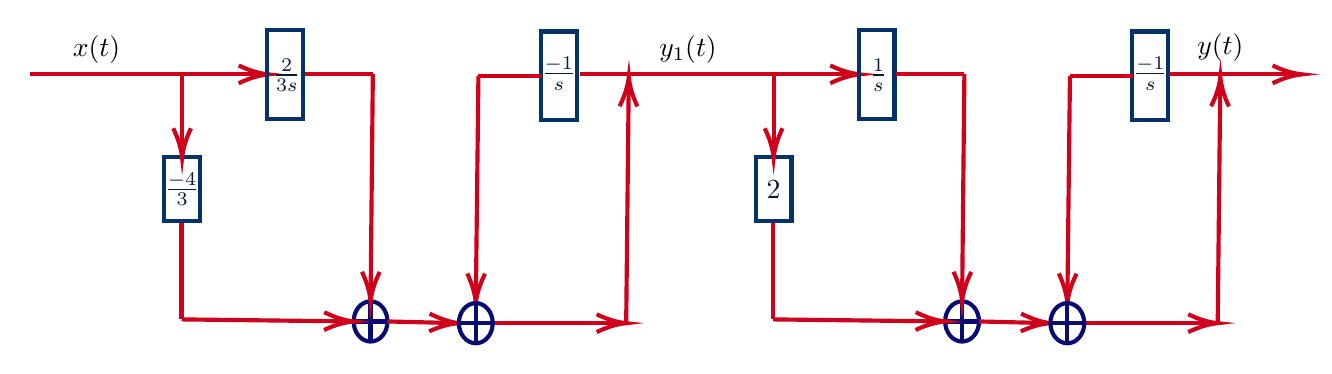
\begin{tikzpicture}[x=0.75pt,y=0.75pt,yscale=-1,xscale=1]
%uncomment if require: \path (0,413); %set diagram left start at 0, and has height of 413

%Straight Lines [id:da5727032991915001] 
\draw [color={rgb, 255:red, 208; green, 2; blue, 27 }  ,draw opacity=1 ][line width=1.5]    (280,98.43) -- (381.28,98.43) ;
%Straight Lines [id:da6353712181396247] 
\draw [color={rgb, 255:red, 208; green, 2; blue, 27 }  ,draw opacity=1 ][line width=1.5]    (381.28,98.43) -- (411.89,98.43) ;
\draw [shift={(414.89,98.43)}, rotate = 180] [color={rgb, 255:red, 208; green, 2; blue, 27 }  ,draw opacity=1 ][line width=1.5]    (14.21,-4.28) .. controls (9.04,-1.82) and (4.3,-0.39) .. (0,0) .. controls (4.3,0.39) and (9.04,1.82) .. (14.21,4.28)   ;
%Straight Lines [id:da5829042456704695] 
\draw [color={rgb, 255:red, 208; green, 2; blue, 27 }  ,draw opacity=1 ][line width=1.5]    (523.06,218.31) -- (584.36,218.31) ;
\draw [shift={(587.36,218.31)}, rotate = 180] [color={rgb, 255:red, 208; green, 2; blue, 27 }  ,draw opacity=1 ][line width=1.5]    (14.21,-4.28) .. controls (9.04,-1.82) and (4.3,-0.39) .. (0,0) .. controls (4.3,0.39) and (9.04,1.82) .. (14.21,4.28)   ;
%Shape: Rectangle [id:dp2516520568905628] 
\draw  [color={rgb, 255:red, 4; green, 51; blue, 104 }  ,draw opacity=1 ][line width=1.5]  (546.25,77.78) -- (563.47,77.78) -- (563.47,120.58) -- (546.25,120.58) -- cycle ;
%Straight Lines [id:da4261405254199824] 
\draw [color={rgb, 255:red, 208; green, 2; blue, 27 }  ,draw opacity=1 ][line width=1.5]    (563.7,98.43) -- (625,98.43) ;
\draw [shift={(628,98.43)}, rotate = 180] [color={rgb, 255:red, 208; green, 2; blue, 27 }  ,draw opacity=1 ][line width=1.5]    (14.21,-4.28) .. controls (9.04,-1.82) and (4.3,-0.39) .. (0,0) .. controls (4.3,0.39) and (9.04,1.82) .. (14.21,4.28)   ;
%Shape: Rectangle [id:dp1355970092994433] 
\draw  [color={rgb, 255:red, 4; green, 51; blue, 104 }  ,draw opacity=1 ][line width=1.5]  (364.79,138.43) -- (382.02,138.43) -- (382.02,169.05) -- (364.79,169.05) -- cycle ;
%Flowchart: Or [id:dp7661436109510428] 
\draw  [color={rgb, 255:red, 7; green, 11; blue, 114 }  ,draw opacity=1 ][line width=1.5]  (456.05,217.48) .. controls (456.05,212.13) and (459.7,207.79) .. (464.2,207.79) .. controls (468.7,207.79) and (472.35,212.13) .. (472.35,217.48) .. controls (472.35,222.82) and (468.7,227.16) .. (464.2,227.16) .. controls (459.7,227.16) and (456.05,222.82) .. (456.05,217.48) -- cycle ; \draw  [color={rgb, 255:red, 7; green, 11; blue, 114 }  ,draw opacity=1 ][line width=1.5]  (456.05,217.48) -- (472.35,217.48) ; \draw  [color={rgb, 255:red, 7; green, 11; blue, 114 }  ,draw opacity=1 ][line width=1.5]  (464.2,207.79) -- (464.2,227.16) ;
%Straight Lines [id:da4878156257526778] 
\draw [color={rgb, 255:red, 208; green, 2; blue, 27 }  ,draw opacity=1 ][line width=1.5]    (503.75,218.24) -- (472.35,217.48) ;
\draw [shift={(506.75,218.31)}, rotate = 181.4] [color={rgb, 255:red, 208; green, 2; blue, 27 }  ,draw opacity=1 ][line width=1.5]    (14.21,-4.28) .. controls (9.04,-1.82) and (4.3,-0.39) .. (0,0) .. controls (4.3,0.39) and (9.04,1.82) .. (14.21,4.28)   ;
%Straight Lines [id:da01710459462168179] 
\draw [color={rgb, 255:red, 208; green, 2; blue, 27 }  ,draw opacity=1 ][line width=1.5]    (453.05,217.44) -- (373.13,216.49) ;
\draw [shift={(456.05,217.48)}, rotate = 180.68] [color={rgb, 255:red, 208; green, 2; blue, 27 }  ,draw opacity=1 ][line width=1.5]    (14.21,-4.28) .. controls (9.04,-1.82) and (4.3,-0.39) .. (0,0) .. controls (4.3,0.39) and (9.04,1.82) .. (14.21,4.28)   ;
%Straight Lines [id:da46828292830077667] 
\draw [color={rgb, 255:red, 208; green, 2; blue, 27 }  ,draw opacity=1 ][line width=1.5]    (373.13,216.49) -- (373.13,170.22) ;
%Shape: Rectangle [id:dp706545784774389] 
\draw  [color={rgb, 255:red, 4; green, 51; blue, 104 }  ,draw opacity=1 ][line width=1.5]  (414.39,76.94) -- (431.62,76.94) -- (431.62,119.74) -- (414.39,119.74) -- cycle ;
%Straight Lines [id:da3449564708681504] 
\draw [color={rgb, 255:red, 208; green, 2; blue, 27 }  ,draw opacity=1 ][line width=1.5]    (373.4,135.63) -- (373.4,99.08) ;
\draw [shift={(373.4,138.63)}, rotate = 270] [color={rgb, 255:red, 208; green, 2; blue, 27 }  ,draw opacity=1 ][line width=1.5]    (14.21,-4.28) .. controls (9.04,-1.82) and (4.3,-0.39) .. (0,0) .. controls (4.3,0.39) and (9.04,1.82) .. (14.21,4.28)   ;
%Straight Lines [id:da5817265537026062] 
\draw [color={rgb, 255:red, 208; green, 2; blue, 27 }  ,draw opacity=1 ][line width=1.5]    (432.48,98.34) -- (465.3,98.34) ;
%Straight Lines [id:da11311142092185089] 
\draw [color={rgb, 255:red, 208; green, 2; blue, 27 }  ,draw opacity=1 ][line width=1.5]    (464.23,204.79) -- (465.3,98.34) ;
\draw [shift={(464.2,207.79)}, rotate = 270.58] [color={rgb, 255:red, 208; green, 2; blue, 27 }  ,draw opacity=1 ][line width=1.5]    (14.21,-4.28) .. controls (9.04,-1.82) and (4.3,-0.39) .. (0,0) .. controls (4.3,0.39) and (9.04,1.82) .. (14.21,4.28)   ;
%Straight Lines [id:da794510001898227] 
\draw [color={rgb, 255:red, 208; green, 2; blue, 27 }  ,draw opacity=1 ][line width=1.5]    (546.62,99.18) -- (516.17,99.18) ;
%Straight Lines [id:da7140545147772185] 
\draw [color={rgb, 255:red, 208; green, 2; blue, 27 }  ,draw opacity=1 ][line width=1.5]    (514.94,205.63) -- (516.17,99.18) ;
\draw [shift={(514.91,208.63)}, rotate = 270.66] [color={rgb, 255:red, 208; green, 2; blue, 27 }  ,draw opacity=1 ][line width=1.5]    (14.21,-4.28) .. controls (9.04,-1.82) and (4.3,-0.39) .. (0,0) .. controls (4.3,0.39) and (9.04,1.82) .. (14.21,4.28)   ;
%Flowchart: Or [id:dp9740541329325205] 
\draw  [color={rgb, 255:red, 7; green, 11; blue, 114 }  ,draw opacity=1 ][line width=1.5]  (506.75,218.31) .. controls (506.75,212.97) and (510.4,208.63) .. (514.91,208.63) .. controls (519.41,208.63) and (523.06,212.97) .. (523.06,218.31) .. controls (523.06,223.66) and (519.41,228) .. (514.91,228) .. controls (510.4,228) and (506.75,223.66) .. (506.75,218.31) -- cycle ; \draw  [color={rgb, 255:red, 7; green, 11; blue, 114 }  ,draw opacity=1 ][line width=1.5]  (506.75,218.31) -- (523.06,218.31) ; \draw  [color={rgb, 255:red, 7; green, 11; blue, 114 }  ,draw opacity=1 ][line width=1.5]  (514.91,208.63) -- (514.91,228) ;
%Straight Lines [id:da8593286249198595] 
\draw [color={rgb, 255:red, 208; green, 2; blue, 27 }  ,draw opacity=1 ][line width=1.5]    (588.59,102.63) -- (587.36,218.31) ;
\draw [shift={(588.63,99.63)}, rotate = 90.61] [color={rgb, 255:red, 208; green, 2; blue, 27 }  ,draw opacity=1 ][line width=1.5]    (14.21,-4.28) .. controls (9.04,-1.82) and (4.3,-0.39) .. (0,0) .. controls (4.3,0.39) and (9.04,1.82) .. (14.21,4.28)   ;
%Straight Lines [id:da07404379893249147] 
\draw [color={rgb, 255:red, 208; green, 2; blue, 27 }  ,draw opacity=1 ][line width=1.5]    (15,98.43) -- (96.28,98.43) ;
%Straight Lines [id:da29437602412680575] 
\draw [color={rgb, 255:red, 208; green, 2; blue, 27 }  ,draw opacity=1 ][line width=1.5]    (96.28,98.43) -- (126.89,98.43) ;
\draw [shift={(129.89,98.43)}, rotate = 180] [color={rgb, 255:red, 208; green, 2; blue, 27 }  ,draw opacity=1 ][line width=1.5]    (14.21,-4.28) .. controls (9.04,-1.82) and (4.3,-0.39) .. (0,0) .. controls (4.3,0.39) and (9.04,1.82) .. (14.21,4.28)   ;
%Straight Lines [id:da6345599707952067] 
\draw [color={rgb, 255:red, 208; green, 2; blue, 27 }  ,draw opacity=1 ][line width=1.5]    (238.06,218.31) -- (299.36,218.31) ;
\draw [shift={(302.36,218.31)}, rotate = 180] [color={rgb, 255:red, 208; green, 2; blue, 27 }  ,draw opacity=1 ][line width=1.5]    (14.21,-4.28) .. controls (9.04,-1.82) and (4.3,-0.39) .. (0,0) .. controls (4.3,0.39) and (9.04,1.82) .. (14.21,4.28)   ;
%Shape: Rectangle [id:dp2551429258382908] 
\draw  [color={rgb, 255:red, 4; green, 51; blue, 104 }  ,draw opacity=1 ][line width=1.5]  (261.25,77.78) -- (278.47,77.78) -- (278.47,120.58) -- (261.25,120.58) -- cycle ;
%Shape: Rectangle [id:dp49046930556068125] 
\draw  [color={rgb, 255:red, 4; green, 51; blue, 104 }  ,draw opacity=1 ][line width=1.5]  (79.79,138.43) -- (97.02,138.43) -- (97.02,169.05) -- (79.79,169.05) -- cycle ;
%Flowchart: Or [id:dp9577467762085949] 
\draw  [color={rgb, 255:red, 7; green, 11; blue, 114 }  ,draw opacity=1 ][line width=1.5]  (171.05,217.48) .. controls (171.05,212.13) and (174.7,207.79) .. (179.2,207.79) .. controls (183.7,207.79) and (187.35,212.13) .. (187.35,217.48) .. controls (187.35,222.82) and (183.7,227.16) .. (179.2,227.16) .. controls (174.7,227.16) and (171.05,222.82) .. (171.05,217.48) -- cycle ; \draw  [color={rgb, 255:red, 7; green, 11; blue, 114 }  ,draw opacity=1 ][line width=1.5]  (171.05,217.48) -- (187.35,217.48) ; \draw  [color={rgb, 255:red, 7; green, 11; blue, 114 }  ,draw opacity=1 ][line width=1.5]  (179.2,207.79) -- (179.2,227.16) ;
%Straight Lines [id:da20276361331041437] 
\draw [color={rgb, 255:red, 208; green, 2; blue, 27 }  ,draw opacity=1 ][line width=1.5]    (218.75,218.24) -- (187.35,217.48) ;
\draw [shift={(221.75,218.31)}, rotate = 181.4] [color={rgb, 255:red, 208; green, 2; blue, 27 }  ,draw opacity=1 ][line width=1.5]    (14.21,-4.28) .. controls (9.04,-1.82) and (4.3,-0.39) .. (0,0) .. controls (4.3,0.39) and (9.04,1.82) .. (14.21,4.28)   ;
%Straight Lines [id:da00896910065208778] 
\draw [color={rgb, 255:red, 208; green, 2; blue, 27 }  ,draw opacity=1 ][line width=1.5]    (168.05,217.44) -- (88.13,216.49) ;
\draw [shift={(171.05,217.48)}, rotate = 180.68] [color={rgb, 255:red, 208; green, 2; blue, 27 }  ,draw opacity=1 ][line width=1.5]    (14.21,-4.28) .. controls (9.04,-1.82) and (4.3,-0.39) .. (0,0) .. controls (4.3,0.39) and (9.04,1.82) .. (14.21,4.28)   ;
%Straight Lines [id:da4031449514760006] 
\draw [color={rgb, 255:red, 208; green, 2; blue, 27 }  ,draw opacity=1 ][line width=1.5]    (88.13,216.49) -- (88.13,170.22) ;
%Shape: Rectangle [id:dp12828817163949235] 
\draw  [color={rgb, 255:red, 4; green, 51; blue, 104 }  ,draw opacity=1 ][line width=1.5]  (129.39,76.94) -- (146.62,76.94) -- (146.62,119.74) -- (129.39,119.74) -- cycle ;
%Straight Lines [id:da5108643254145206] 
\draw [color={rgb, 255:red, 208; green, 2; blue, 27 }  ,draw opacity=1 ][line width=1.5]    (88.4,135.63) -- (88.4,99.08) ;
\draw [shift={(88.4,138.63)}, rotate = 270] [color={rgb, 255:red, 208; green, 2; blue, 27 }  ,draw opacity=1 ][line width=1.5]    (14.21,-4.28) .. controls (9.04,-1.82) and (4.3,-0.39) .. (0,0) .. controls (4.3,0.39) and (9.04,1.82) .. (14.21,4.28)   ;
%Straight Lines [id:da5509593799503646] 
\draw [color={rgb, 255:red, 208; green, 2; blue, 27 }  ,draw opacity=1 ][line width=1.5]    (147.48,98.34) -- (180.3,98.34) ;
%Straight Lines [id:da6055205952316761] 
\draw [color={rgb, 255:red, 208; green, 2; blue, 27 }  ,draw opacity=1 ][line width=1.5]    (179.23,204.79) -- (180.3,98.34) ;
\draw [shift={(179.2,207.79)}, rotate = 270.58] [color={rgb, 255:red, 208; green, 2; blue, 27 }  ,draw opacity=1 ][line width=1.5]    (14.21,-4.28) .. controls (9.04,-1.82) and (4.3,-0.39) .. (0,0) .. controls (4.3,0.39) and (9.04,1.82) .. (14.21,4.28)   ;
%Straight Lines [id:da30980150913282456] 
\draw [color={rgb, 255:red, 208; green, 2; blue, 27 }  ,draw opacity=1 ][line width=1.5]    (261.62,99.18) -- (231.17,99.18) ;
%Straight Lines [id:da668026193955427] 
\draw [color={rgb, 255:red, 208; green, 2; blue, 27 }  ,draw opacity=1 ][line width=1.5]    (229.94,205.63) -- (231.17,99.18) ;
\draw [shift={(229.91,208.63)}, rotate = 270.66] [color={rgb, 255:red, 208; green, 2; blue, 27 }  ,draw opacity=1 ][line width=1.5]    (14.21,-4.28) .. controls (9.04,-1.82) and (4.3,-0.39) .. (0,0) .. controls (4.3,0.39) and (9.04,1.82) .. (14.21,4.28)   ;
%Flowchart: Or [id:dp8258028344065087] 
\draw  [color={rgb, 255:red, 7; green, 11; blue, 114 }  ,draw opacity=1 ][line width=1.5]  (221.75,218.31) .. controls (221.75,212.97) and (225.4,208.63) .. (229.91,208.63) .. controls (234.41,208.63) and (238.06,212.97) .. (238.06,218.31) .. controls (238.06,223.66) and (234.41,228) .. (229.91,228) .. controls (225.4,228) and (221.75,223.66) .. (221.75,218.31) -- cycle ; \draw  [color={rgb, 255:red, 7; green, 11; blue, 114 }  ,draw opacity=1 ][line width=1.5]  (221.75,218.31) -- (238.06,218.31) ; \draw  [color={rgb, 255:red, 7; green, 11; blue, 114 }  ,draw opacity=1 ][line width=1.5]  (229.91,208.63) -- (229.91,228) ;
%Straight Lines [id:da02937626456625375] 
\draw [color={rgb, 255:red, 208; green, 2; blue, 27 }  ,draw opacity=1 ][line width=1.5]    (303.59,102.63) -- (302.36,218.31) ;
\draw [shift={(303.63,99.63)}, rotate = 90.61] [color={rgb, 255:red, 208; green, 2; blue, 27 }  ,draw opacity=1 ][line width=1.5]    (14.21,-4.28) .. controls (9.04,-1.82) and (4.3,-0.39) .. (0,0) .. controls (4.3,0.39) and (9.04,1.82) .. (14.21,4.28)   ;

% Text Node
\draw (332.15,94.45) node [anchor=south] [inner sep=0.75pt]    {$y_{1}( t)$};
% Text Node
\draw (423.82,98.75) node  [color={rgb, 255:red, 5; green, 27; blue, 53 }  ,opacity=1 ]  {$\frac{1}{s}$};
% Text Node
\draw (554.86,98.12) node  [color={rgb, 255:red, 5; green, 27; blue, 53 }  ,opacity=1 ]  {$\frac{-1}{s}$};
% Text Node
\draw (588.63,93.48) node [anchor=south] [inner sep=0.75pt]    {$y( t)$};
% Text Node
\draw (373.4,153.74) node  [color={rgb, 255:red, 5; green, 27; blue, 53 }  ,opacity=1 ]  {$2$};
% Text Node
\draw (47.15,94.45) node [anchor=south] [inner sep=0.75pt]    {$x( t)$};
% Text Node
\draw (138.82,98.75) node  [color={rgb, 255:red, 5; green, 27; blue, 53 }  ,opacity=1 ]  {$\frac{2}{3s}$};
% Text Node
\draw (269.86,98.12) node  [color={rgb, 255:red, 5; green, 27; blue, 53 }  ,opacity=1 ]  {$\frac{-1}{s}$};
% Text Node
\draw (88.4,153.74) node  [color={rgb, 255:red, 5; green, 27; blue, 53 }  ,opacity=1 ]  {$\frac{-4}{3}$};


\end{tikzpicture}

          \caption{Representation of Full System, $H(s)$}
          \label{fig:4}
        \end{figure}

      \item Based on the given system, we may obtain:

        \begin{figure}[H]
          \centering
          \tikzset{every picture/.style={line width=0.75pt}} %set default line width to 0.75pt        

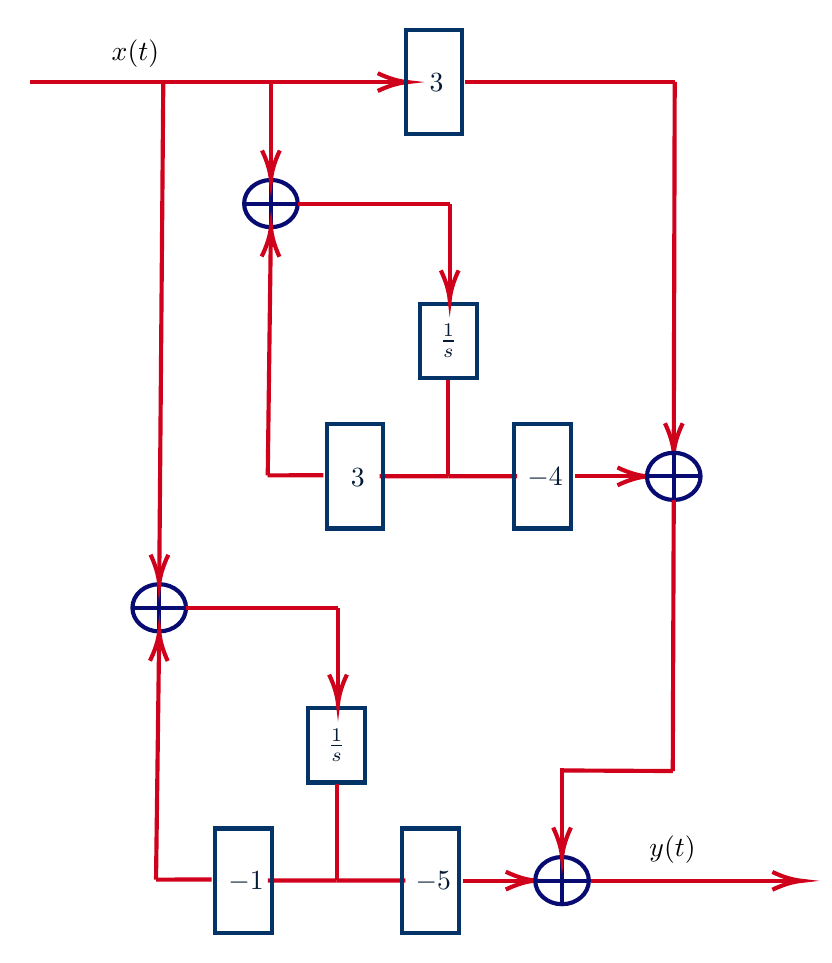
\begin{tikzpicture}[x=0.75pt,y=0.75pt,yscale=-1,xscale=1]
%uncomment if require: \path (0,590); %set diagram left start at 0, and has height of 590

%Straight Lines [id:da4261405254199824] 
\draw [color={rgb, 255:red, 208; green, 2; blue, 27 }  ,draw opacity=1 ][line width=1.5]    (285.22,487) -- (384,487) ;
\draw [shift={(387,487)}, rotate = 180] [color={rgb, 255:red, 208; green, 2; blue, 27 }  ,draw opacity=1 ][line width=1.5]    (14.21,-4.28) .. controls (9.04,-1.82) and (4.3,-0.39) .. (0,0) .. controls (4.3,0.39) and (9.04,1.82) .. (14.21,4.28)   ;
%Straight Lines [id:da07404379893249147] 
\draw [color={rgb, 255:red, 208; green, 2; blue, 27 }  ,draw opacity=1 ][line width=1.5]    (15,102.17) -- (143.67,102.17) ;
%Straight Lines [id:da29437602412680575] 
\draw [color={rgb, 255:red, 208; green, 2; blue, 27 }  ,draw opacity=1 ][line width=1.5]    (143.67,102.17) -- (193.87,102.17) ;
\draw [shift={(196.87,102.17)}, rotate = 180] [color={rgb, 255:red, 208; green, 2; blue, 27 }  ,draw opacity=1 ][line width=1.5]    (14.21,-4.28) .. controls (9.04,-1.82) and (4.3,-0.39) .. (0,0) .. controls (4.3,0.39) and (9.04,1.82) .. (14.21,4.28)   ;
%Shape: Rectangle [id:dp49046930556068125] 
\draw  [color={rgb, 255:red, 4; green, 51; blue, 104 }  ,draw opacity=1 ][line width=1.5]  (203.04,208.93) -- (230.32,208.93) -- (230.32,244.86) -- (203.04,244.86) -- cycle ;
%Flowchart: Or [id:dp9577467762085949] 
\draw  [color={rgb, 255:red, 7; green, 11; blue, 114 }  ,draw opacity=1 ][line width=1.5]  (118.29,160.7) .. controls (118.29,154.42) and (124.07,149.33) .. (131.2,149.33) .. controls (138.33,149.33) and (144.11,154.42) .. (144.11,160.7) .. controls (144.11,166.97) and (138.33,172.06) .. (131.2,172.06) .. controls (124.07,172.06) and (118.29,166.97) .. (118.29,160.7) -- cycle ; \draw  [color={rgb, 255:red, 7; green, 11; blue, 114 }  ,draw opacity=1 ][line width=1.5]  (118.29,160.7) -- (144.11,160.7) ; \draw  [color={rgb, 255:red, 7; green, 11; blue, 114 }  ,draw opacity=1 ][line width=1.5]  (131.2,149.33) -- (131.2,172.06) ;
%Straight Lines [id:da00896910065208778] 
\draw [color={rgb, 255:red, 208; green, 2; blue, 27 }  ,draw opacity=1 ][line width=1.5]    (309.37,292.13) -- (277.79,292.13) ;
\draw [shift={(312.37,292.13)}, rotate = 180] [color={rgb, 255:red, 208; green, 2; blue, 27 }  ,draw opacity=1 ][line width=1.5]    (14.21,-4.28) .. controls (9.04,-1.82) and (4.3,-0.39) .. (0,0) .. controls (4.3,0.39) and (9.04,1.82) .. (14.21,4.28)   ;
%Straight Lines [id:da4031449514760006] 
\draw [color={rgb, 255:red, 208; green, 2; blue, 27 }  ,draw opacity=1 ][line width=1.5]    (144.11,160.7) -- (217.34,160.7) ;
%Shape: Rectangle [id:dp12828817163949235] 
\draw  [color={rgb, 255:red, 4; green, 51; blue, 104 }  ,draw opacity=1 ][line width=1.5]  (196.08,76.95) -- (223.36,76.95) -- (223.36,127.17) -- (196.08,127.17) -- cycle ;
%Straight Lines [id:da5108643254145206] 
\draw [color={rgb, 255:red, 208; green, 2; blue, 27 }  ,draw opacity=1 ][line width=1.5]    (131.2,146.33) -- (131.2,102.93) ;
\draw [shift={(131.2,149.33)}, rotate = 270] [color={rgb, 255:red, 208; green, 2; blue, 27 }  ,draw opacity=1 ][line width=1.5]    (14.21,-4.28) .. controls (9.04,-1.82) and (4.3,-0.39) .. (0,0) .. controls (4.3,0.39) and (9.04,1.82) .. (14.21,4.28)   ;
%Straight Lines [id:da5509593799503646] 
\draw [color={rgb, 255:red, 208; green, 2; blue, 27 }  ,draw opacity=1 ][line width=1.5]    (224.72,102.06) -- (325.74,102.06) ;
%Straight Lines [id:da6055205952316761] 
\draw [color={rgb, 255:red, 208; green, 2; blue, 27 }  ,draw opacity=1 ][line width=1.5]    (325.29,277.76) -- (325.74,102.06) ;
\draw [shift={(325.28,280.76)}, rotate = 270.15] [color={rgb, 255:red, 208; green, 2; blue, 27 }  ,draw opacity=1 ][line width=1.5]    (14.21,-4.28) .. controls (9.04,-1.82) and (4.3,-0.39) .. (0,0) .. controls (4.3,0.39) and (9.04,1.82) .. (14.21,4.28)   ;
%Straight Lines [id:da07460124765912668] 
\draw [color={rgb, 255:red, 208; green, 2; blue, 27 }  ,draw opacity=1 ][line width=1.5]    (217.34,204.1) -- (217.34,160.7) ;
\draw [shift={(217.34,207.1)}, rotate = 270] [color={rgb, 255:red, 208; green, 2; blue, 27 }  ,draw opacity=1 ][line width=1.5]    (14.21,-4.28) .. controls (9.04,-1.82) and (4.3,-0.39) .. (0,0) .. controls (4.3,0.39) and (9.04,1.82) .. (14.21,4.28)   ;
%Straight Lines [id:da3425780609164075] 
\draw [color={rgb, 255:red, 208; green, 2; blue, 27 }  ,draw opacity=1 ][line width=1.5]    (216.68,292.07) -- (216.68,245.67) ;
%Straight Lines [id:da16626408866649778] 
\draw [color={rgb, 255:red, 208; green, 2; blue, 27 }  ,draw opacity=1 ][line width=1.5]    (183.57,292.1) -- (216.68,292.07) ;
%Straight Lines [id:da800776487296986] 
\draw [color={rgb, 255:red, 208; green, 2; blue, 27 }  ,draw opacity=1 ][line width=1.5]    (131.16,175.06) -- (129.66,291.64) ;
\draw [shift={(131.2,172.06)}, rotate = 90.74] [color={rgb, 255:red, 208; green, 2; blue, 27 }  ,draw opacity=1 ][line width=1.5]    (14.21,-4.28) .. controls (9.04,-1.82) and (4.3,-0.39) .. (0,0) .. controls (4.3,0.39) and (9.04,1.82) .. (14.21,4.28)   ;
%Shape: Rectangle [id:dp5221741522085411] 
\draw  [color={rgb, 255:red, 4; green, 51; blue, 104 }  ,draw opacity=1 ][line width=1.5]  (158.09,267.02) -- (185.37,267.02) -- (185.37,317.24) -- (158.09,317.24) -- cycle ;
%Straight Lines [id:da44526725560798674] 
\draw [color={rgb, 255:red, 208; green, 2; blue, 27 }  ,draw opacity=1 ][line width=1.5]    (129.66,291.64) -- (156.44,291.6) ;
%Straight Lines [id:da6592414618049504] 
\draw [color={rgb, 255:red, 208; green, 2; blue, 27 }  ,draw opacity=1 ][line width=1.5]    (216.68,292.07) -- (249.79,292.04) ;
%Shape: Rectangle [id:dp6159769523993353] 
\draw  [color={rgb, 255:red, 4; green, 51; blue, 104 }  ,draw opacity=1 ][line width=1.5]  (248.32,267.02) -- (275.6,267.02) -- (275.6,317.24) -- (248.32,317.24) -- cycle ;
%Flowchart: Or [id:dp44737778976530074] 
\draw  [color={rgb, 255:red, 7; green, 11; blue, 114 }  ,draw opacity=1 ][line width=1.5]  (312.37,292.13) .. controls (312.37,285.85) and (318.15,280.76) .. (325.28,280.76) .. controls (332.41,280.76) and (338.19,285.85) .. (338.19,292.13) .. controls (338.19,298.4) and (332.41,303.49) .. (325.28,303.49) .. controls (318.15,303.49) and (312.37,298.4) .. (312.37,292.13) -- cycle ; \draw  [color={rgb, 255:red, 7; green, 11; blue, 114 }  ,draw opacity=1 ][line width=1.5]  (312.37,292.13) -- (338.19,292.13) ; \draw  [color={rgb, 255:red, 7; green, 11; blue, 114 }  ,draw opacity=1 ][line width=1.5]  (325.28,280.76) -- (325.28,303.49) ;
%Shape: Rectangle [id:dp24578410589477728] 
\draw  [color={rgb, 255:red, 4; green, 51; blue, 104 }  ,draw opacity=1 ][line width=1.5]  (149.22,403.69) -- (176.49,403.69) -- (176.49,439.62) -- (149.22,439.62) -- cycle ;
%Flowchart: Or [id:dp6998267702859198] 
\draw  [color={rgb, 255:red, 7; green, 11; blue, 114 }  ,draw opacity=1 ][line width=1.5]  (64.47,355.46) .. controls (64.47,349.18) and (70.25,344.1) .. (77.38,344.1) .. controls (84.51,344.1) and (90.28,349.18) .. (90.28,355.46) .. controls (90.28,361.74) and (84.51,366.82) .. (77.38,366.82) .. controls (70.25,366.82) and (64.47,361.74) .. (64.47,355.46) -- cycle ; \draw  [color={rgb, 255:red, 7; green, 11; blue, 114 }  ,draw opacity=1 ][line width=1.5]  (64.47,355.46) -- (90.28,355.46) ; \draw  [color={rgb, 255:red, 7; green, 11; blue, 114 }  ,draw opacity=1 ][line width=1.5]  (77.38,344.1) -- (77.38,366.82) ;
%Straight Lines [id:da971976885313287] 
\draw [color={rgb, 255:red, 208; green, 2; blue, 27 }  ,draw opacity=1 ][line width=1.5]    (255.55,486.89) -- (223.97,486.89) ;
\draw [shift={(258.55,486.89)}, rotate = 180] [color={rgb, 255:red, 208; green, 2; blue, 27 }  ,draw opacity=1 ][line width=1.5]    (14.21,-4.28) .. controls (9.04,-1.82) and (4.3,-0.39) .. (0,0) .. controls (4.3,0.39) and (9.04,1.82) .. (14.21,4.28)   ;
%Straight Lines [id:da6931515154882544] 
\draw [color={rgb, 255:red, 208; green, 2; blue, 27 }  ,draw opacity=1 ][line width=1.5]    (163.52,398.86) -- (163.52,355.46) ;
\draw [shift={(163.52,401.86)}, rotate = 270] [color={rgb, 255:red, 208; green, 2; blue, 27 }  ,draw opacity=1 ][line width=1.5]    (14.21,-4.28) .. controls (9.04,-1.82) and (4.3,-0.39) .. (0,0) .. controls (4.3,0.39) and (9.04,1.82) .. (14.21,4.28)   ;
%Straight Lines [id:da7740950137398847] 
\draw [color={rgb, 255:red, 208; green, 2; blue, 27 }  ,draw opacity=1 ][line width=1.5]    (162.86,486.83) -- (162.86,440.43) ;
%Straight Lines [id:da42600262106997655] 
\draw [color={rgb, 255:red, 208; green, 2; blue, 27 }  ,draw opacity=1 ][line width=1.5]    (129.75,486.86) -- (162.86,486.83) ;
%Straight Lines [id:da272216861909394] 
\draw [color={rgb, 255:red, 208; green, 2; blue, 27 }  ,draw opacity=1 ][line width=1.5]    (77.34,369.82) -- (75.84,486.4) ;
\draw [shift={(77.38,366.82)}, rotate = 90.74] [color={rgb, 255:red, 208; green, 2; blue, 27 }  ,draw opacity=1 ][line width=1.5]    (14.21,-4.28) .. controls (9.04,-1.82) and (4.3,-0.39) .. (0,0) .. controls (4.3,0.39) and (9.04,1.82) .. (14.21,4.28)   ;
%Shape: Rectangle [id:dp8526747255851159] 
\draw  [color={rgb, 255:red, 4; green, 51; blue, 104 }  ,draw opacity=1 ][line width=1.5]  (104.27,461.78) -- (131.55,461.78) -- (131.55,512) -- (104.27,512) -- cycle ;
%Straight Lines [id:da12689469422707755] 
\draw [color={rgb, 255:red, 208; green, 2; blue, 27 }  ,draw opacity=1 ][line width=1.5]    (75.84,486.4) -- (102.61,486.37) ;
%Straight Lines [id:da25337789464485305] 
\draw [color={rgb, 255:red, 208; green, 2; blue, 27 }  ,draw opacity=1 ][line width=1.5]    (162.86,486.83) -- (195.97,486.8) ;
%Shape: Rectangle [id:dp2762221190815598] 
\draw  [color={rgb, 255:red, 4; green, 51; blue, 104 }  ,draw opacity=1 ][line width=1.5]  (194.5,461.78) -- (221.77,461.78) -- (221.77,512) -- (194.5,512) -- cycle ;
%Straight Lines [id:da7323098569298919] 
\draw [color={rgb, 255:red, 208; green, 2; blue, 27 }  ,draw opacity=1 ][line width=1.5]    (77.4,341.1) -- (79.34,102.17) ;
\draw [shift={(77.38,344.1)}, rotate = 270.46] [color={rgb, 255:red, 208; green, 2; blue, 27 }  ,draw opacity=1 ][line width=1.5]    (14.21,-4.28) .. controls (9.04,-1.82) and (4.3,-0.39) .. (0,0) .. controls (4.3,0.39) and (9.04,1.82) .. (14.21,4.28)   ;
%Straight Lines [id:da7582438600732586] 
\draw [color={rgb, 255:red, 208; green, 2; blue, 27 }  ,draw opacity=1 ][line width=1.5]    (90.28,355.46) -- (163.52,355.46) ;
%Flowchart: Or [id:dp11380770250352523] 
\draw  [color={rgb, 255:red, 7; green, 11; blue, 114 }  ,draw opacity=1 ][line width=1.5]  (258.55,486.89) .. controls (258.55,480.62) and (264.33,475.53) .. (271.46,475.53) .. controls (278.59,475.53) and (284.36,480.62) .. (284.36,486.89) .. controls (284.36,493.17) and (278.59,498.26) .. (271.46,498.26) .. controls (264.33,498.26) and (258.55,493.17) .. (258.55,486.89) -- cycle ; \draw  [color={rgb, 255:red, 7; green, 11; blue, 114 }  ,draw opacity=1 ][line width=1.5]  (258.55,486.89) -- (284.36,486.89) ; \draw  [color={rgb, 255:red, 7; green, 11; blue, 114 }  ,draw opacity=1 ][line width=1.5]  (271.46,475.53) -- (271.46,498.26) ;
%Straight Lines [id:da047750735099190256] 
\draw [color={rgb, 255:red, 208; green, 2; blue, 27 }  ,draw opacity=1 ][line width=1.5]    (324.81,434.09) -- (325.28,303.49) ;
%Straight Lines [id:da46096543709945337] 
\draw [color={rgb, 255:red, 208; green, 2; blue, 27 }  ,draw opacity=1 ][line width=1.5]    (271.46,433.82) -- (324.81,434.09) ;
%Straight Lines [id:da48723423389880127] 
\draw [color={rgb, 255:red, 208; green, 2; blue, 27 }  ,draw opacity=1 ][line width=1.5]    (271.46,472.53) -- (271.46,432.64) ;
\draw [shift={(271.46,475.53)}, rotate = 270] [color={rgb, 255:red, 208; green, 2; blue, 27 }  ,draw opacity=1 ][line width=1.5]    (14.21,-4.28) .. controls (9.04,-1.82) and (4.3,-0.39) .. (0,0) .. controls (4.3,0.39) and (9.04,1.82) .. (14.21,4.28)   ;

% Text Node
\draw (324.67,479.88) node [anchor=south] [inner sep=0.75pt]    {$y( t)$};
% Text Node
\draw (65.89,96.18) node [anchor=south] [inner sep=0.75pt]    {$x( t)$};
% Text Node
\draw (211,102.54) node  [color={rgb, 255:red, 5; green, 27; blue, 53 }  ,opacity=1 ]  {$3$};
% Text Node
\draw (216.68,226.89) node  [color={rgb, 255:red, 5; green, 27; blue, 53 }  ,opacity=1 ]  {$\frac{1}{s}$};
% Text Node
\draw (173.01,292.61) node  [color={rgb, 255:red, 5; green, 27; blue, 53 }  ,opacity=1 ]  {$3$};
% Text Node
\draw (263.24,292.61) node  [color={rgb, 255:red, 5; green, 27; blue, 53 }  ,opacity=1 ]  {$-4$};
% Text Node
\draw (162.86,421.66) node  [color={rgb, 255:red, 5; green, 27; blue, 53 }  ,opacity=1 ]  {$\frac{1}{s}$};
% Text Node
\draw (119.19,487.37) node  [color={rgb, 255:red, 5; green, 27; blue, 53 }  ,opacity=1 ]  {$-1$};
% Text Node
\draw (209.42,487.37) node  [color={rgb, 255:red, 5; green, 27; blue, 53 }  ,opacity=1 ]  {$-5$};


\end{tikzpicture}

          \caption{Representation of Full System (Part g), $H(s)$}
          \label{fig:5}
        \end{figure}

    \end{enumerate}

  \item

    \begin{enumerate}

      \item We may begin by converting all of the components to the frequency domain:

        $$z_C=\frac{1}{sC}\quad\text{ and }\quad z_L=sL$$

        This gives us:

        $$R=1[\si{\ohm}],\, z_C=\frac{2}{s}[\si{\ohm}],\, z_l=.4s[\si{\ohm}]$$

        Given that the components are in parallel, we can find the equivalent impedance:

        $$z_{eq1}=\frac{z_Cz_L}{z_C+z_L}$$
        $$z_{eq1}=\frac{.8}{(2/s)+.4s}$$
        $$z_{eq1}=\frac{.8s}{2+.4s^2}$$

        And then:

        $$z_{eq}=\frac{Rz_{eq1}}{R+z_{eq1}}$$
        $$z_{eq}=\frac{z_{eq1}}{1+z_{eq1}}$$
        $$z_{eq}=\frac{.8s}{2+.8s+.4s^2}$$

        The voltage through each branch may be found by taking:

        $$v(t)=z_{eq}i_g(t)$$
        $$v(t)=\frac{.8si_g(t)}{2+.8s+.4s^2}$$

        We then divide by the impedance of the capacitor to find the current:

        $$i_o(t)=\frac{.4s^2i_g(t)}{2+.8s+.4s^2}$$

        We then find the transfer function:

        $$H(s)=\frac{i_o(s)}{i_g(t)}$$
        $$H(s)=\frac{.4s^2}{2+.8s+.4s^2}$$

        To simplify, we multiply both the numerator and denominator by 5:

        $$H(s)=\frac{2s^2}{10+4s+2s^2}$$
        $$\boxed{H(s)=\frac{s^2}{5+2s+s^2}}$$

      \item 

        Given that we know:

        $$H(s)=\frac{Y(s)}{X(s)}$$

        We may obtain:

        $$s^2X(s)=[5+2s+s^2]Y(s)$$

        This gives us:

        $$\boxed{\frac{d^2i_g(t)}{dt^2}=5i_o(t)+2\frac{di_o(t)}{dt}+\frac{d^2i_o(t)}{dt^2}}$$

      \item 

        We may obtain $I_o(s)$ using the transfer function:

        $$I_o(s)=\left[ \frac{s^2}{s^2+2s+5} \right]I_g(s)$$

        We take the Laplace transform for the current input to get:

        $$I_g(s)=\frac{10s}{s^2+1}$$

        Multiplying, we get:

        $$\boxed{I_o(s)=\frac{10s^3}{(s^2+1)(s^2+2s+5)}}$$

      \item 

        We may begin by using partial fraction decomposition, such that:

        $$I_o(s)=\frac{As+B}{s^2+1}+\frac{Cs+D}{s^2+2s+5}$$

        Multiplying together, we find:

        $$Cs^3+Cs+Ds^2+D+As^3+2As^2+5As+Bs^2+2Bs+5B=10s^3$$

        This allows us to generate the following system:

        $$C+A=10$$
        $$D+2A+B=0$$
        $$C+5A+2B=0$$
        $$D+5B=0$$

        We solve the system and find: $A=-2, B=-1, C=12$, and $D=5$, which gives us:

        $$I_o(s)=\frac{-2s-1}{s^2+1}+\frac{12s+5}{s^2+2s+5}$$

        Continuing to simplify to take the inverse, we get:

        $$I_o(s)=-\frac{2s+1}{s^2+1}+\frac{12s+5}{(s+1)^2+2^2}$$
        $$I_o(s)=-\frac{2s}{s^2+1}-\frac{1}{s^2+1}+\frac{12(s+1)}{(s+1)^2+2^2}-\frac{7}{(s+1)^2+2^2}$$

        Per our tables, this gives us:

        $$\boxed{i_o(t)=[\underbrace{-2\cos(t)-\sin(t)}_{\text{steady-state}}+\overbrace{12e^{-t}\cos(2t)-7e^{-t}\sin(2t)}^{\text{transient}}]u(t)}$$

        The transient terms fade with time and are expressed as those with decaying exponentials, while the steady state response is purely sinusoidal.

    \end{enumerate}

\end{enumerate}

\end{document}

